\subsection{Start Up}
	\subsection*{\\Required Equipment:\\}
		\begin{itemize}
			\item ReVA Raspberry Pi.
			\item Rasberry Pi charger.
			\item Double adapter.
			\item internet connection.
			\textbf{\\\\For initial set up only: }
			\item Screen.
			\item Mouse.
			\item Keyboard.
			\item VGA to HDMI converter (Depends on screen).

			\item HDMI to HDMI cable or VGA to VGA cable (Depends on screen).

		\end{itemize}
		
		
\begin{figure}[ht!]
\centering
\begin{minipage}{.5\textwidth}
  \centering
 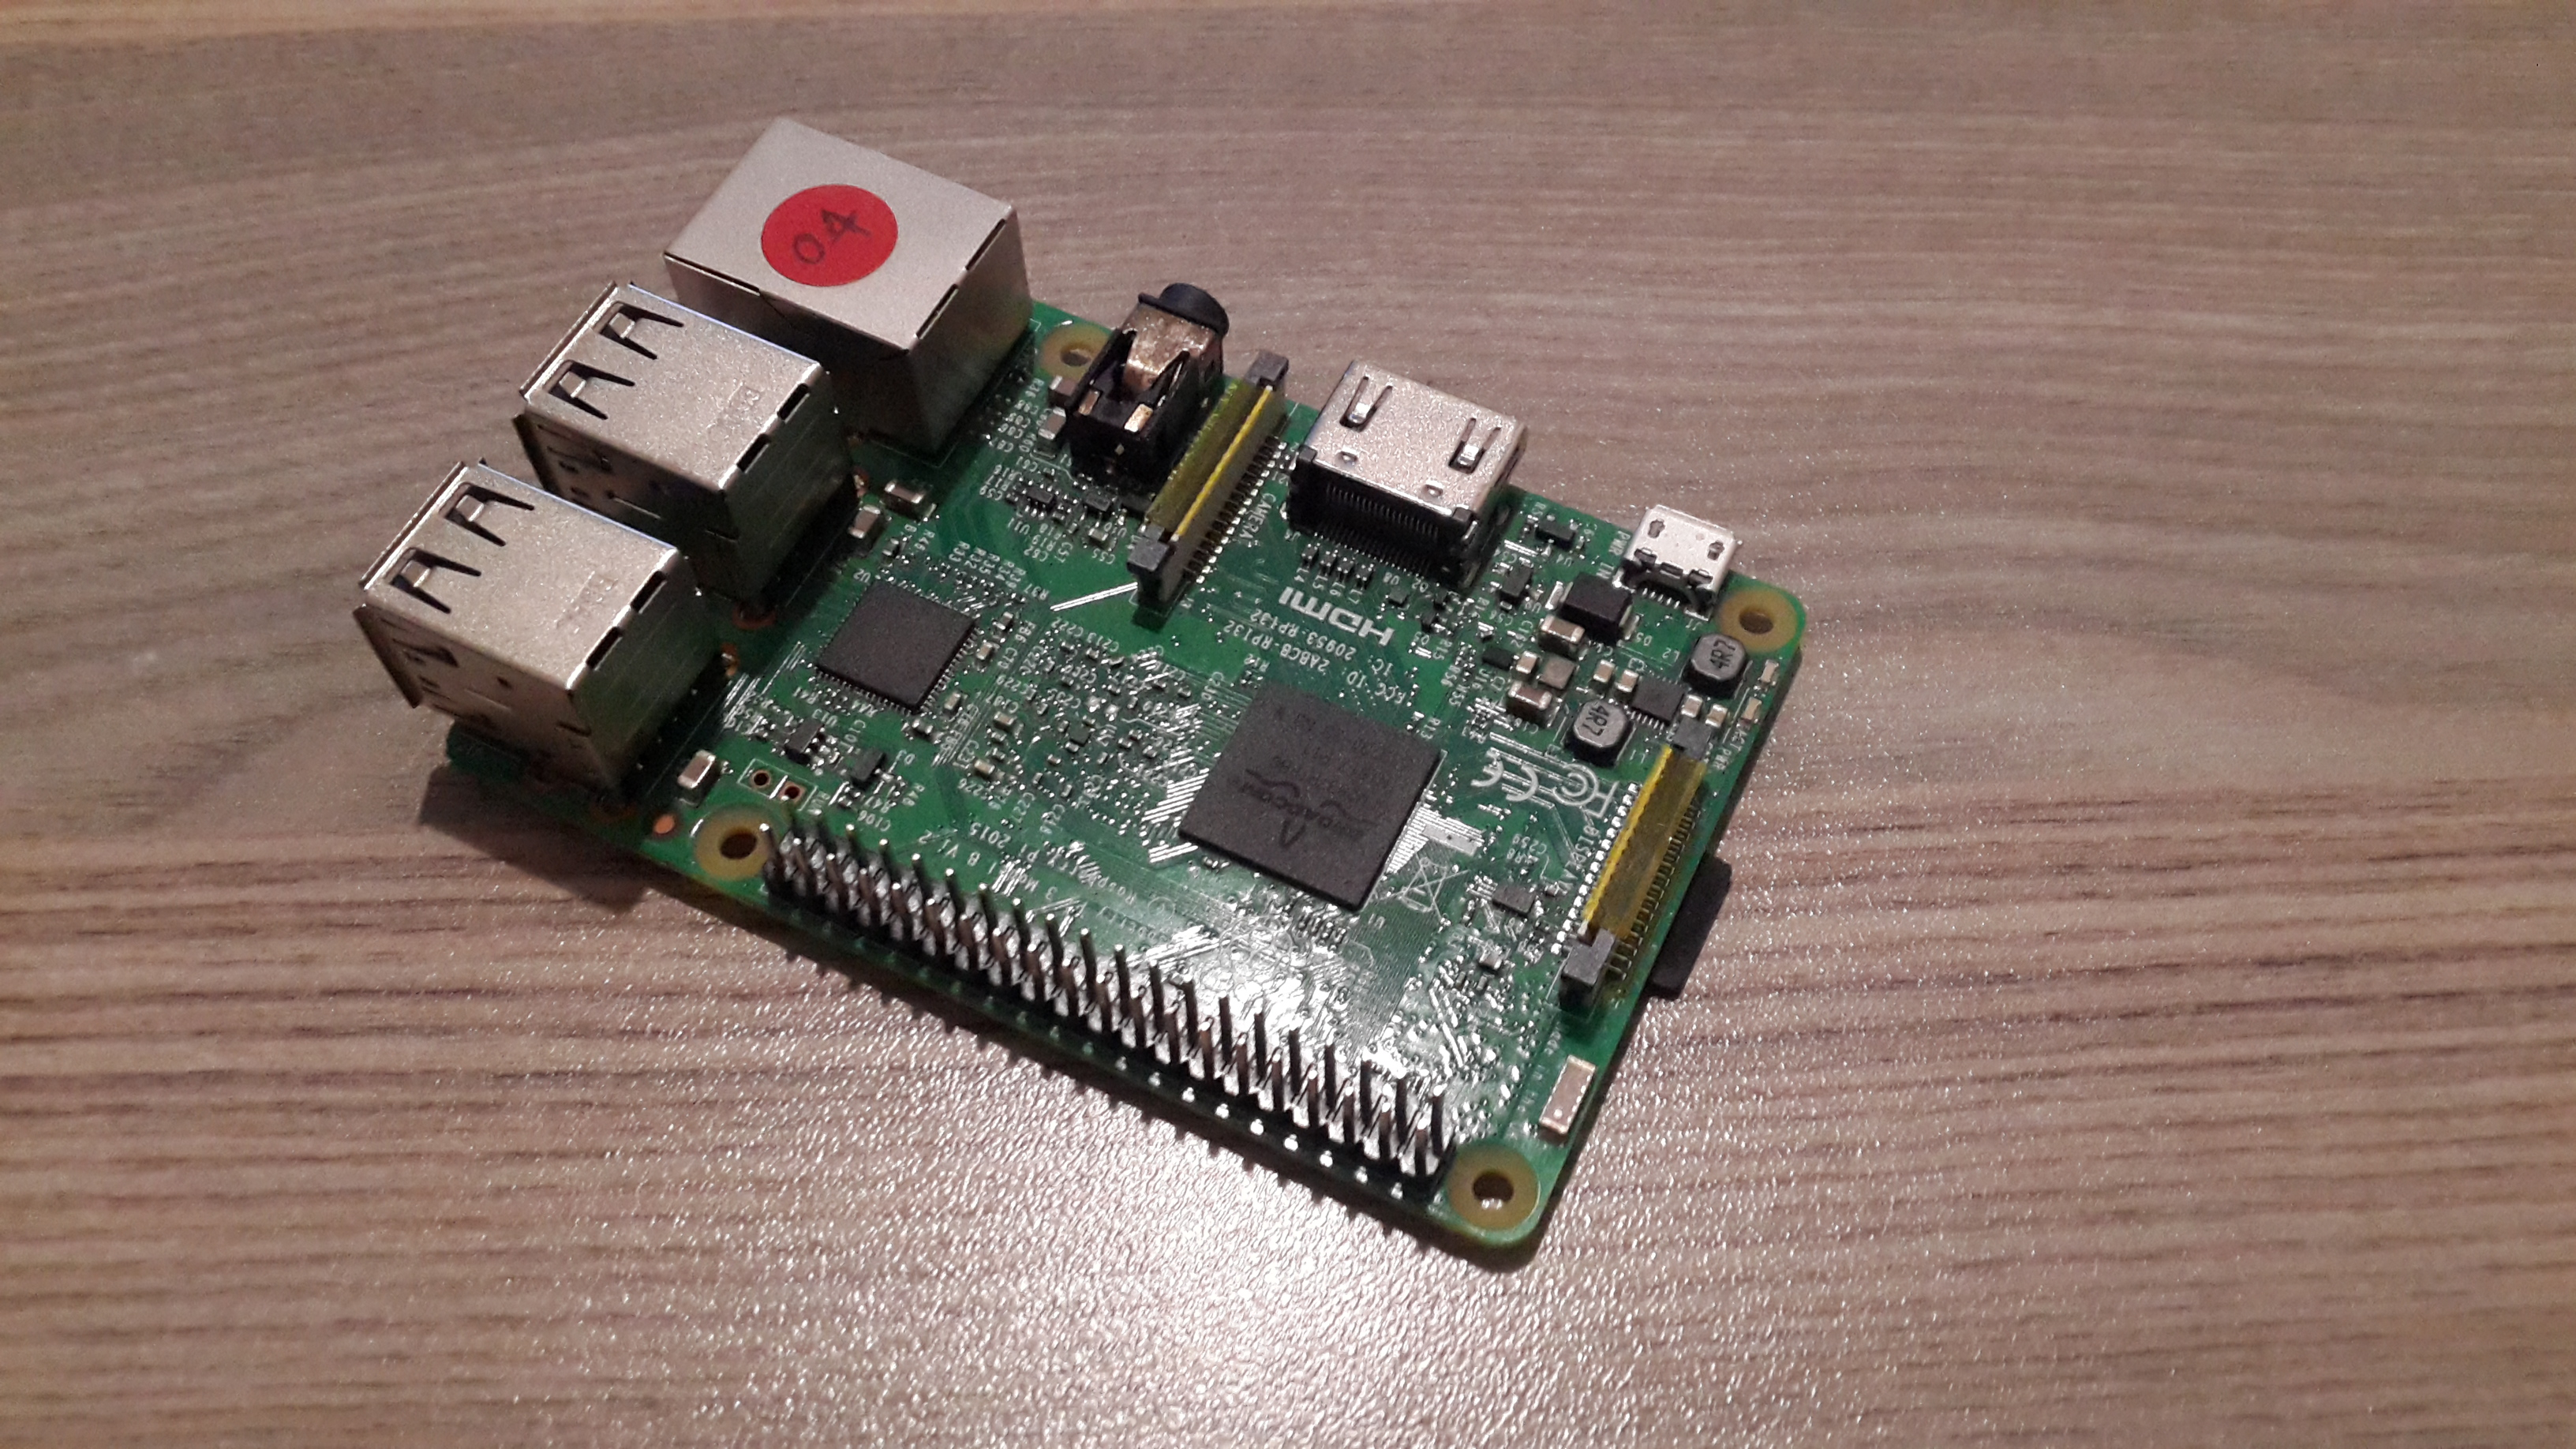
\includegraphics[width=0.9\linewidth]{../images/manual/RPi1.jpg}
  \caption{ Raspberry Pi without cover}

\end{minipage}%
\begin{minipage}{.5\textwidth}
  \centering
 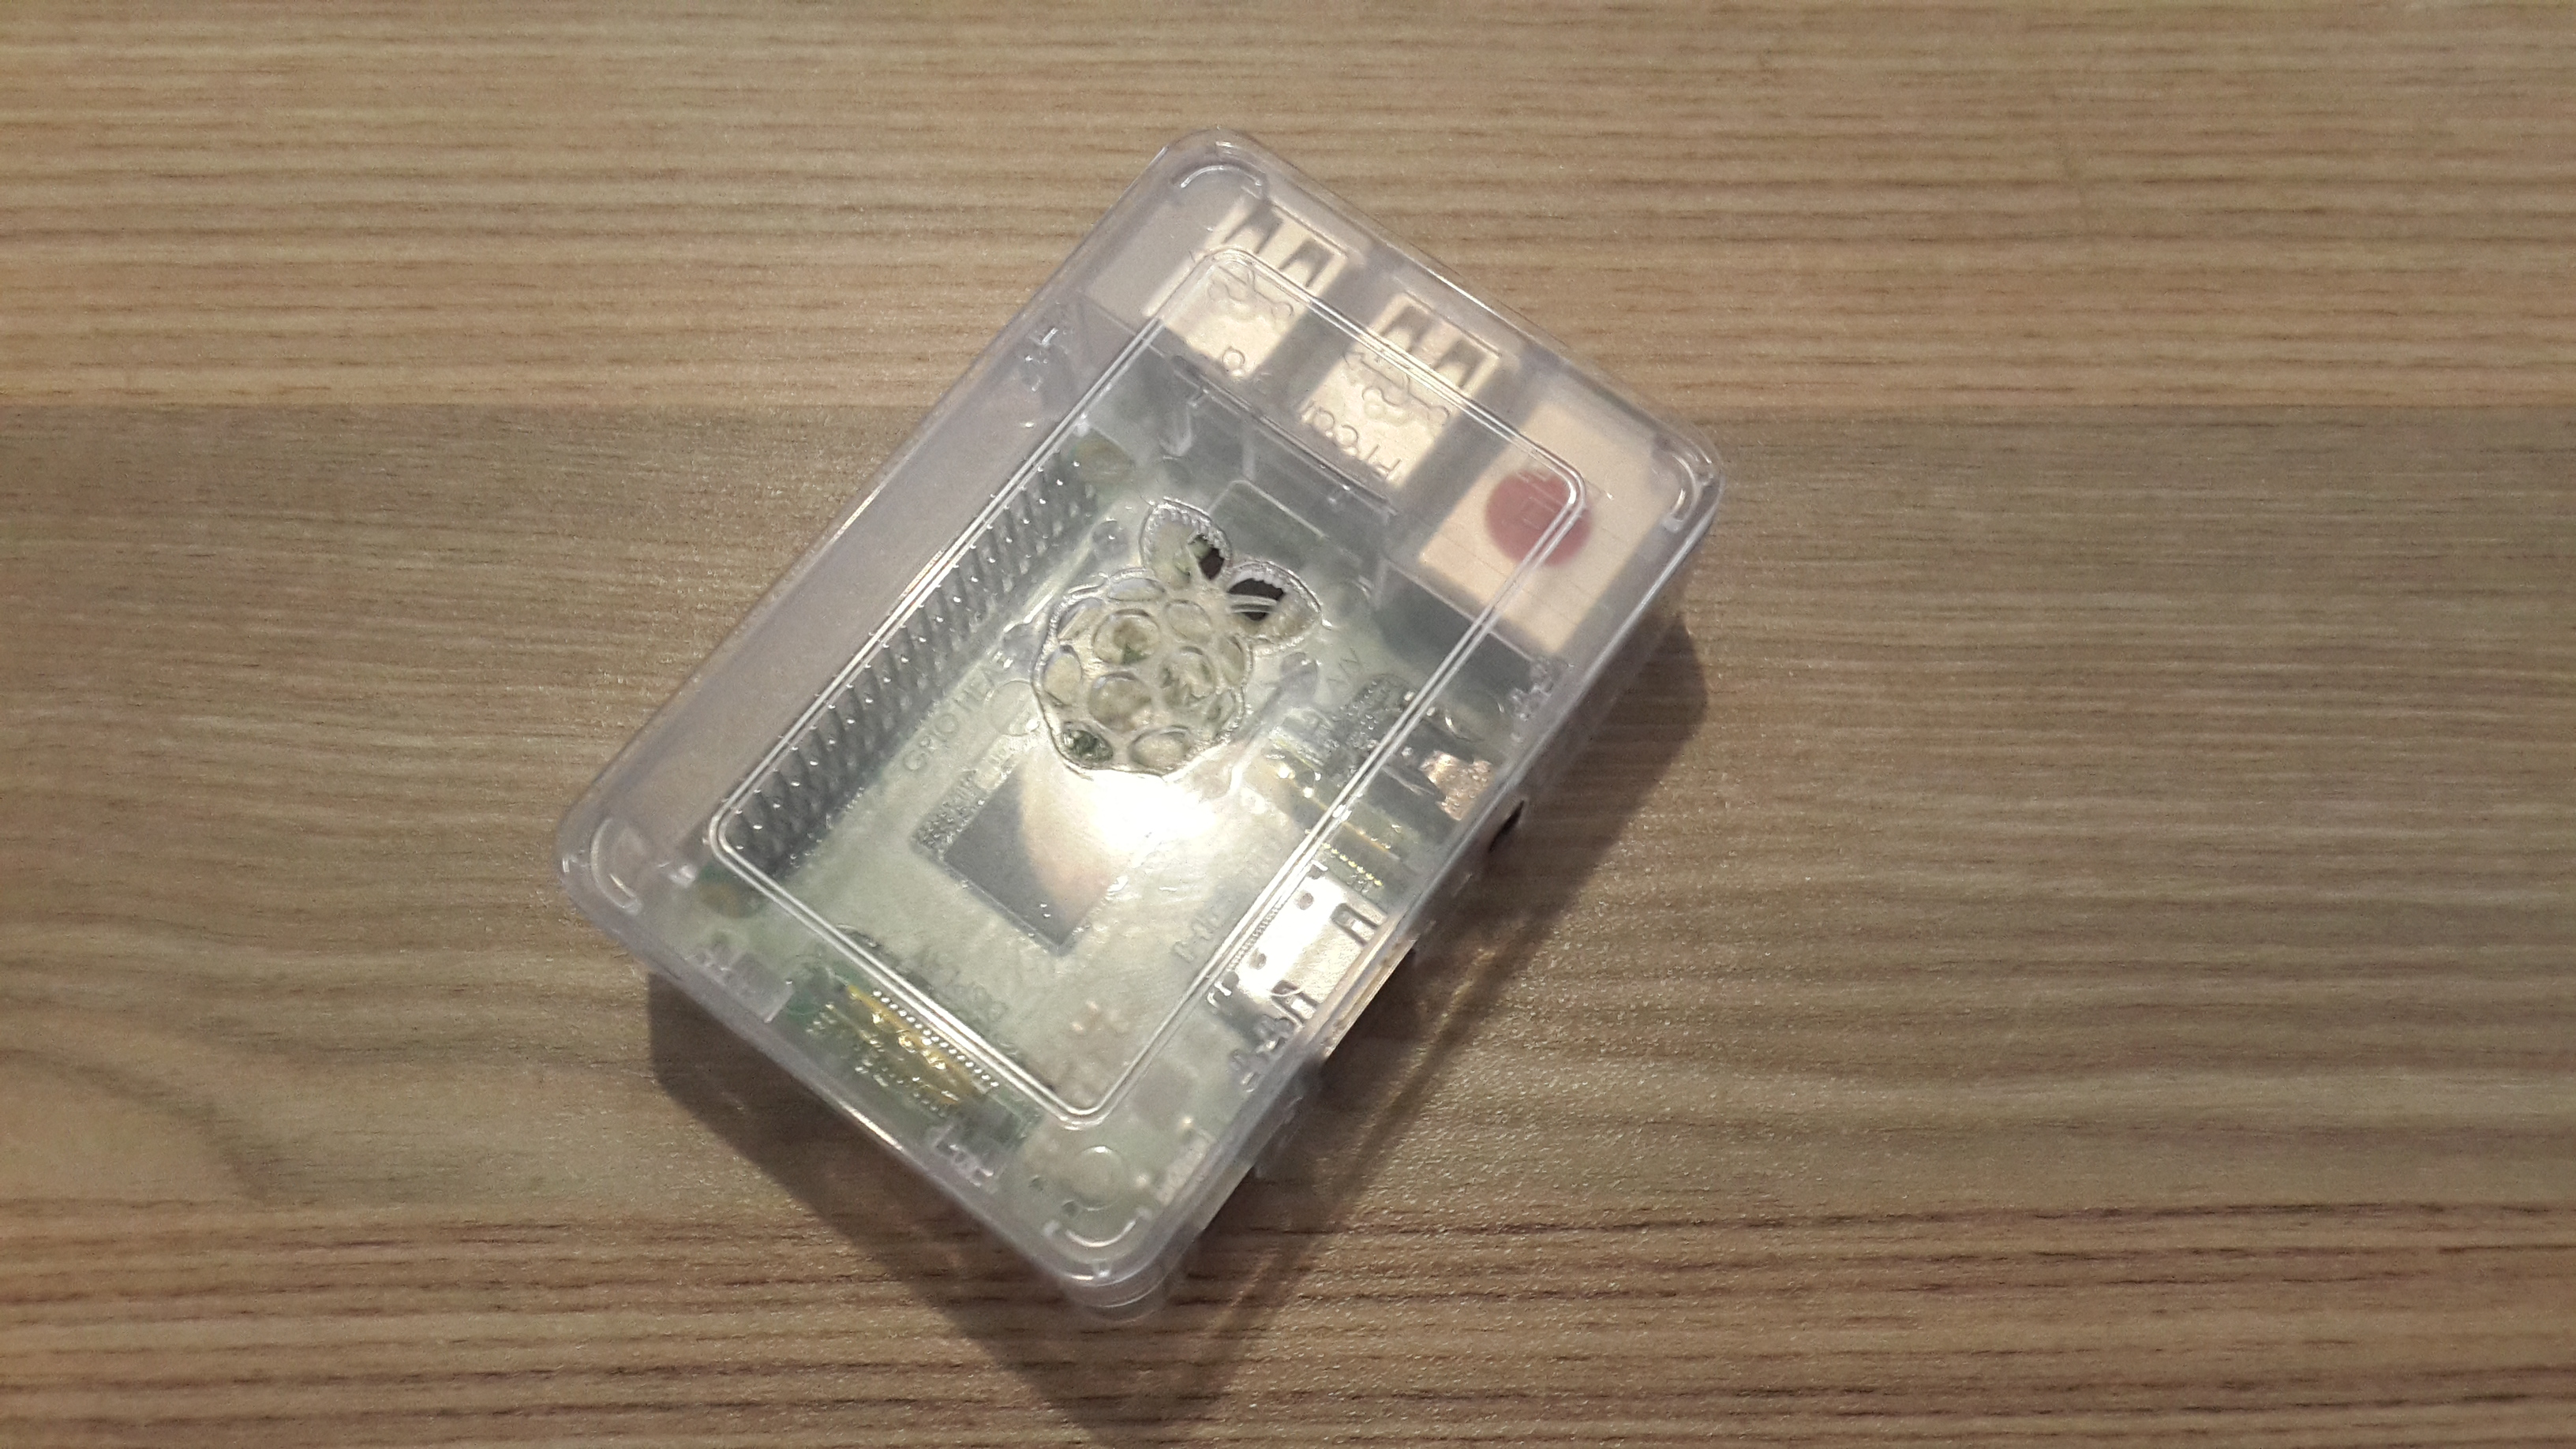
\includegraphics[width=0.9\linewidth]{../images/manual/RPi2.jpg}
  \caption{ Raspberry Pi with cover}
\end{minipage}
\end{figure}


\begin{figure}[ht!]
\centering
\begin{minipage}{.5\textwidth}
  \centering
 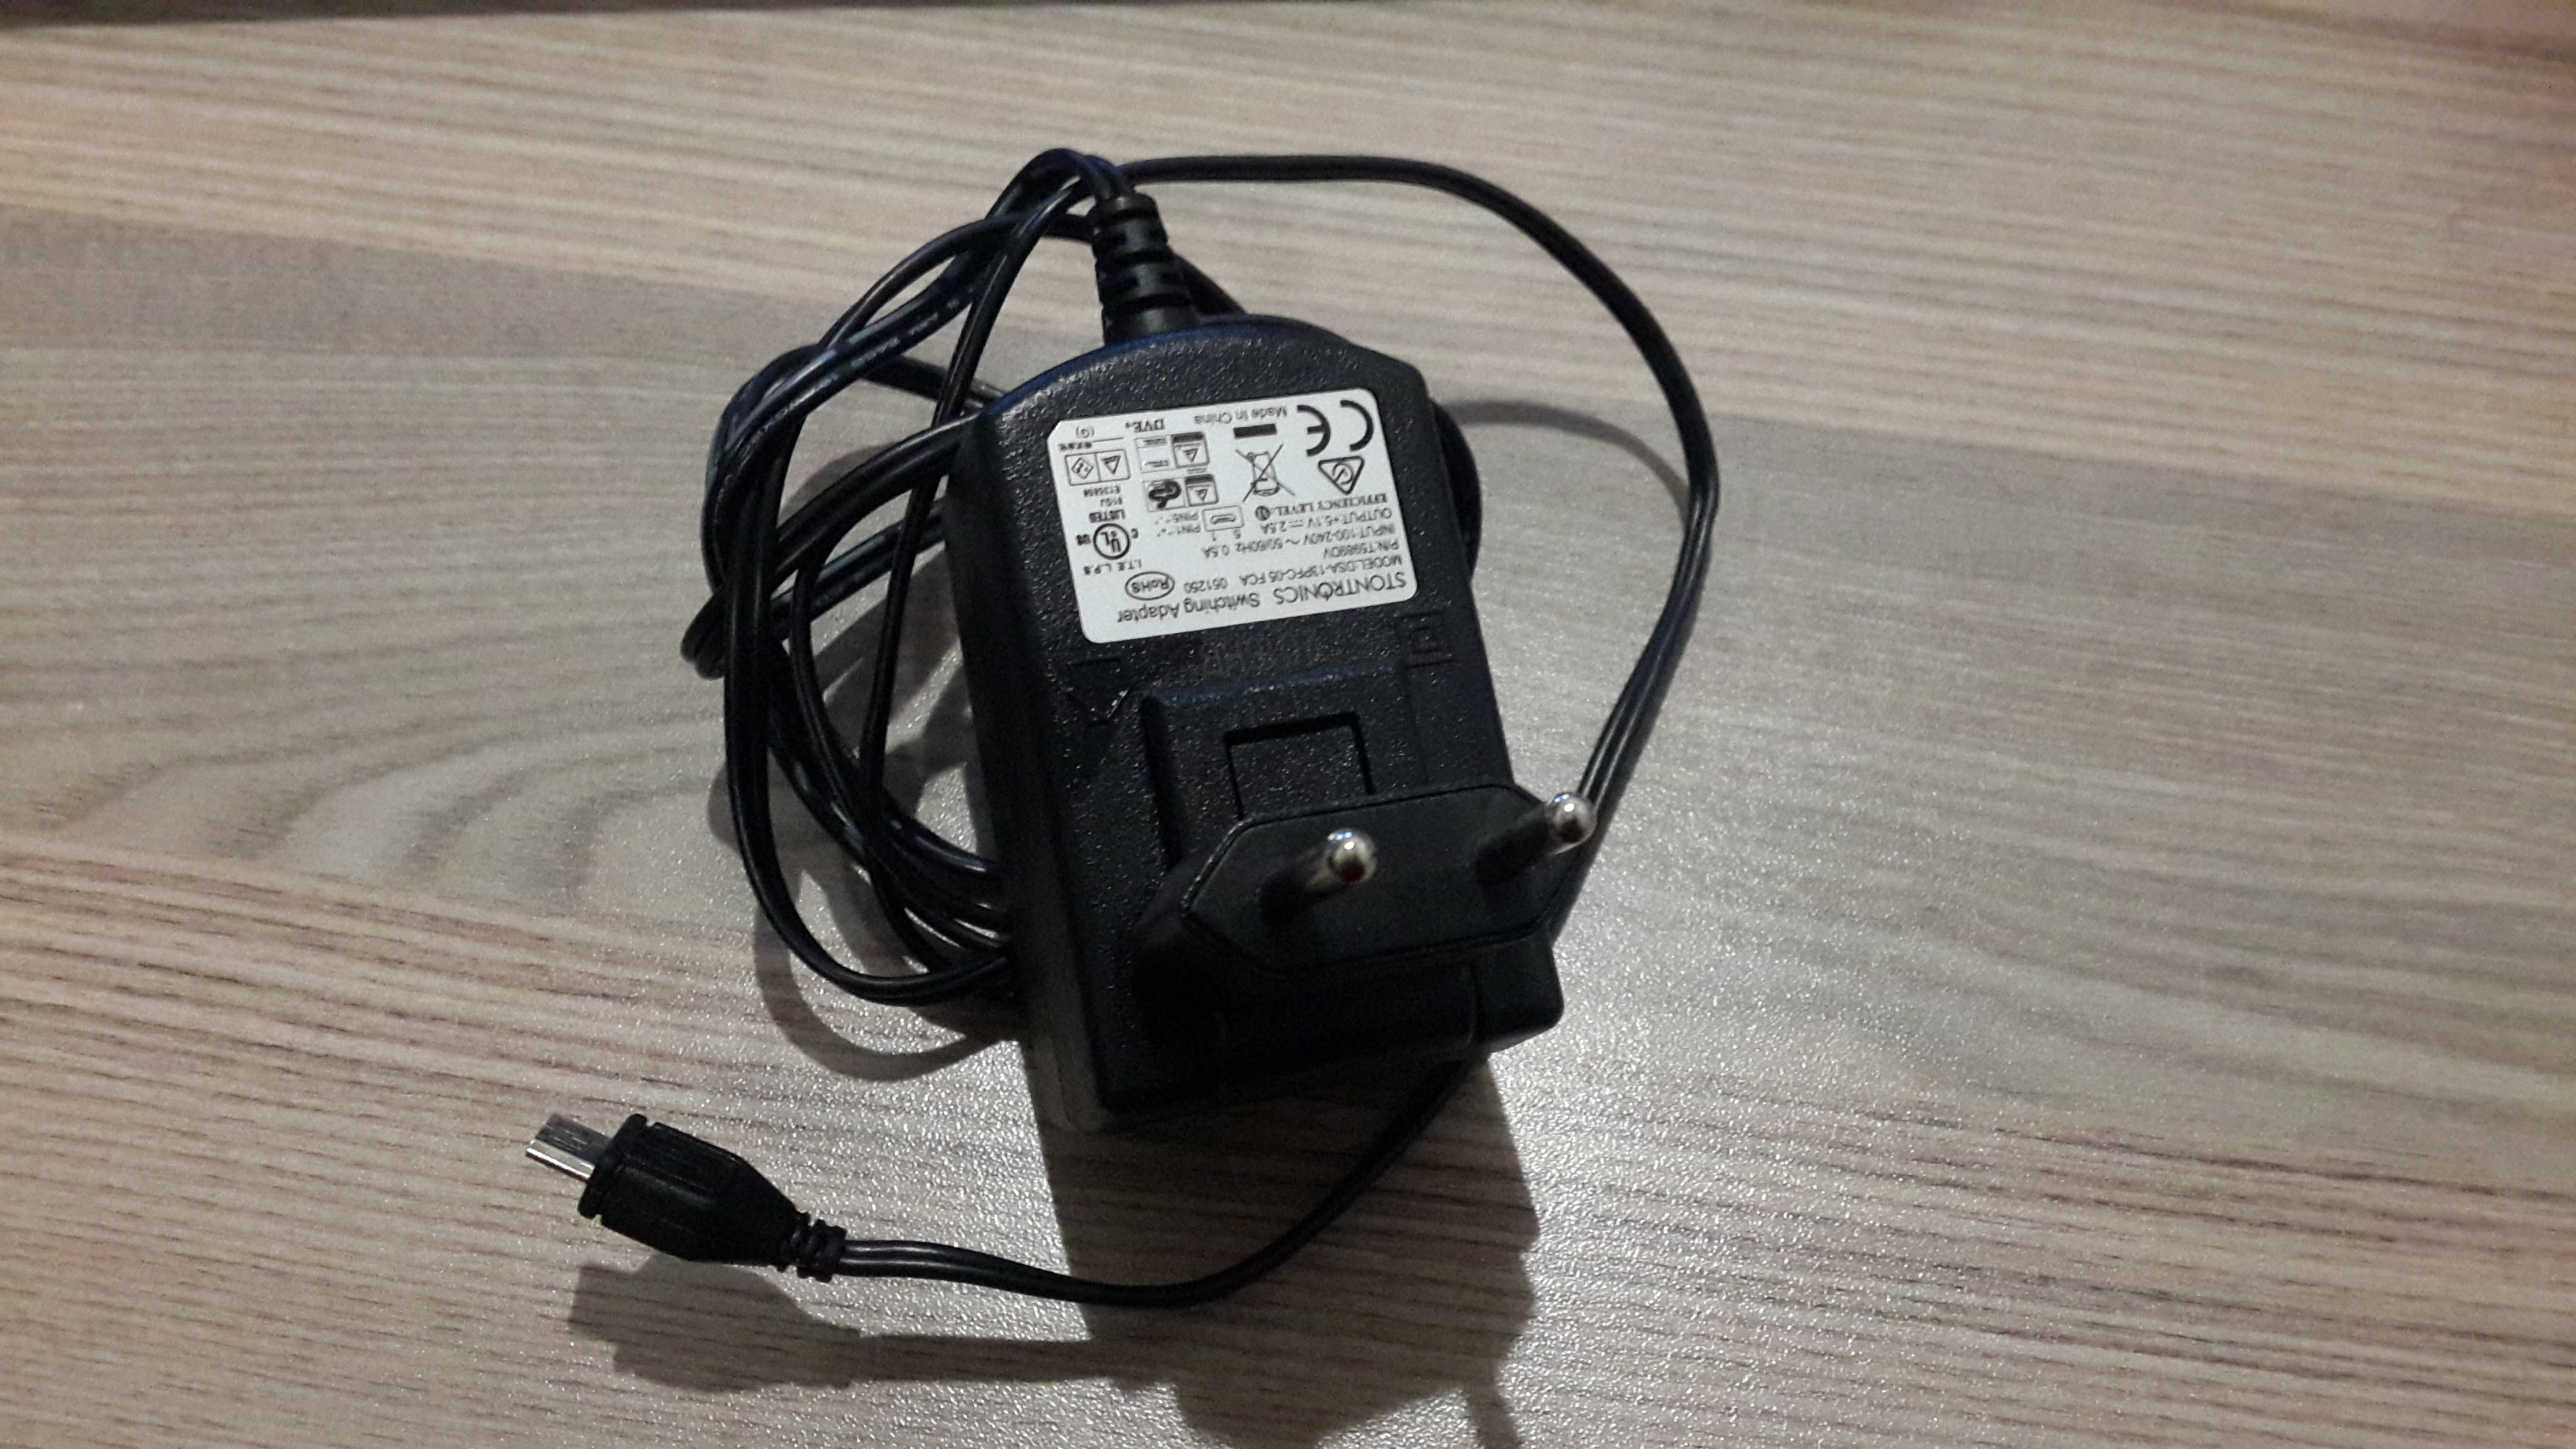
\includegraphics[width=0.9\linewidth]{../images/manual/charger.jpg}
  \caption{ Raspberry Pi charger}

\end{minipage}%
\begin{minipage}{.5\textwidth}
  \centering
  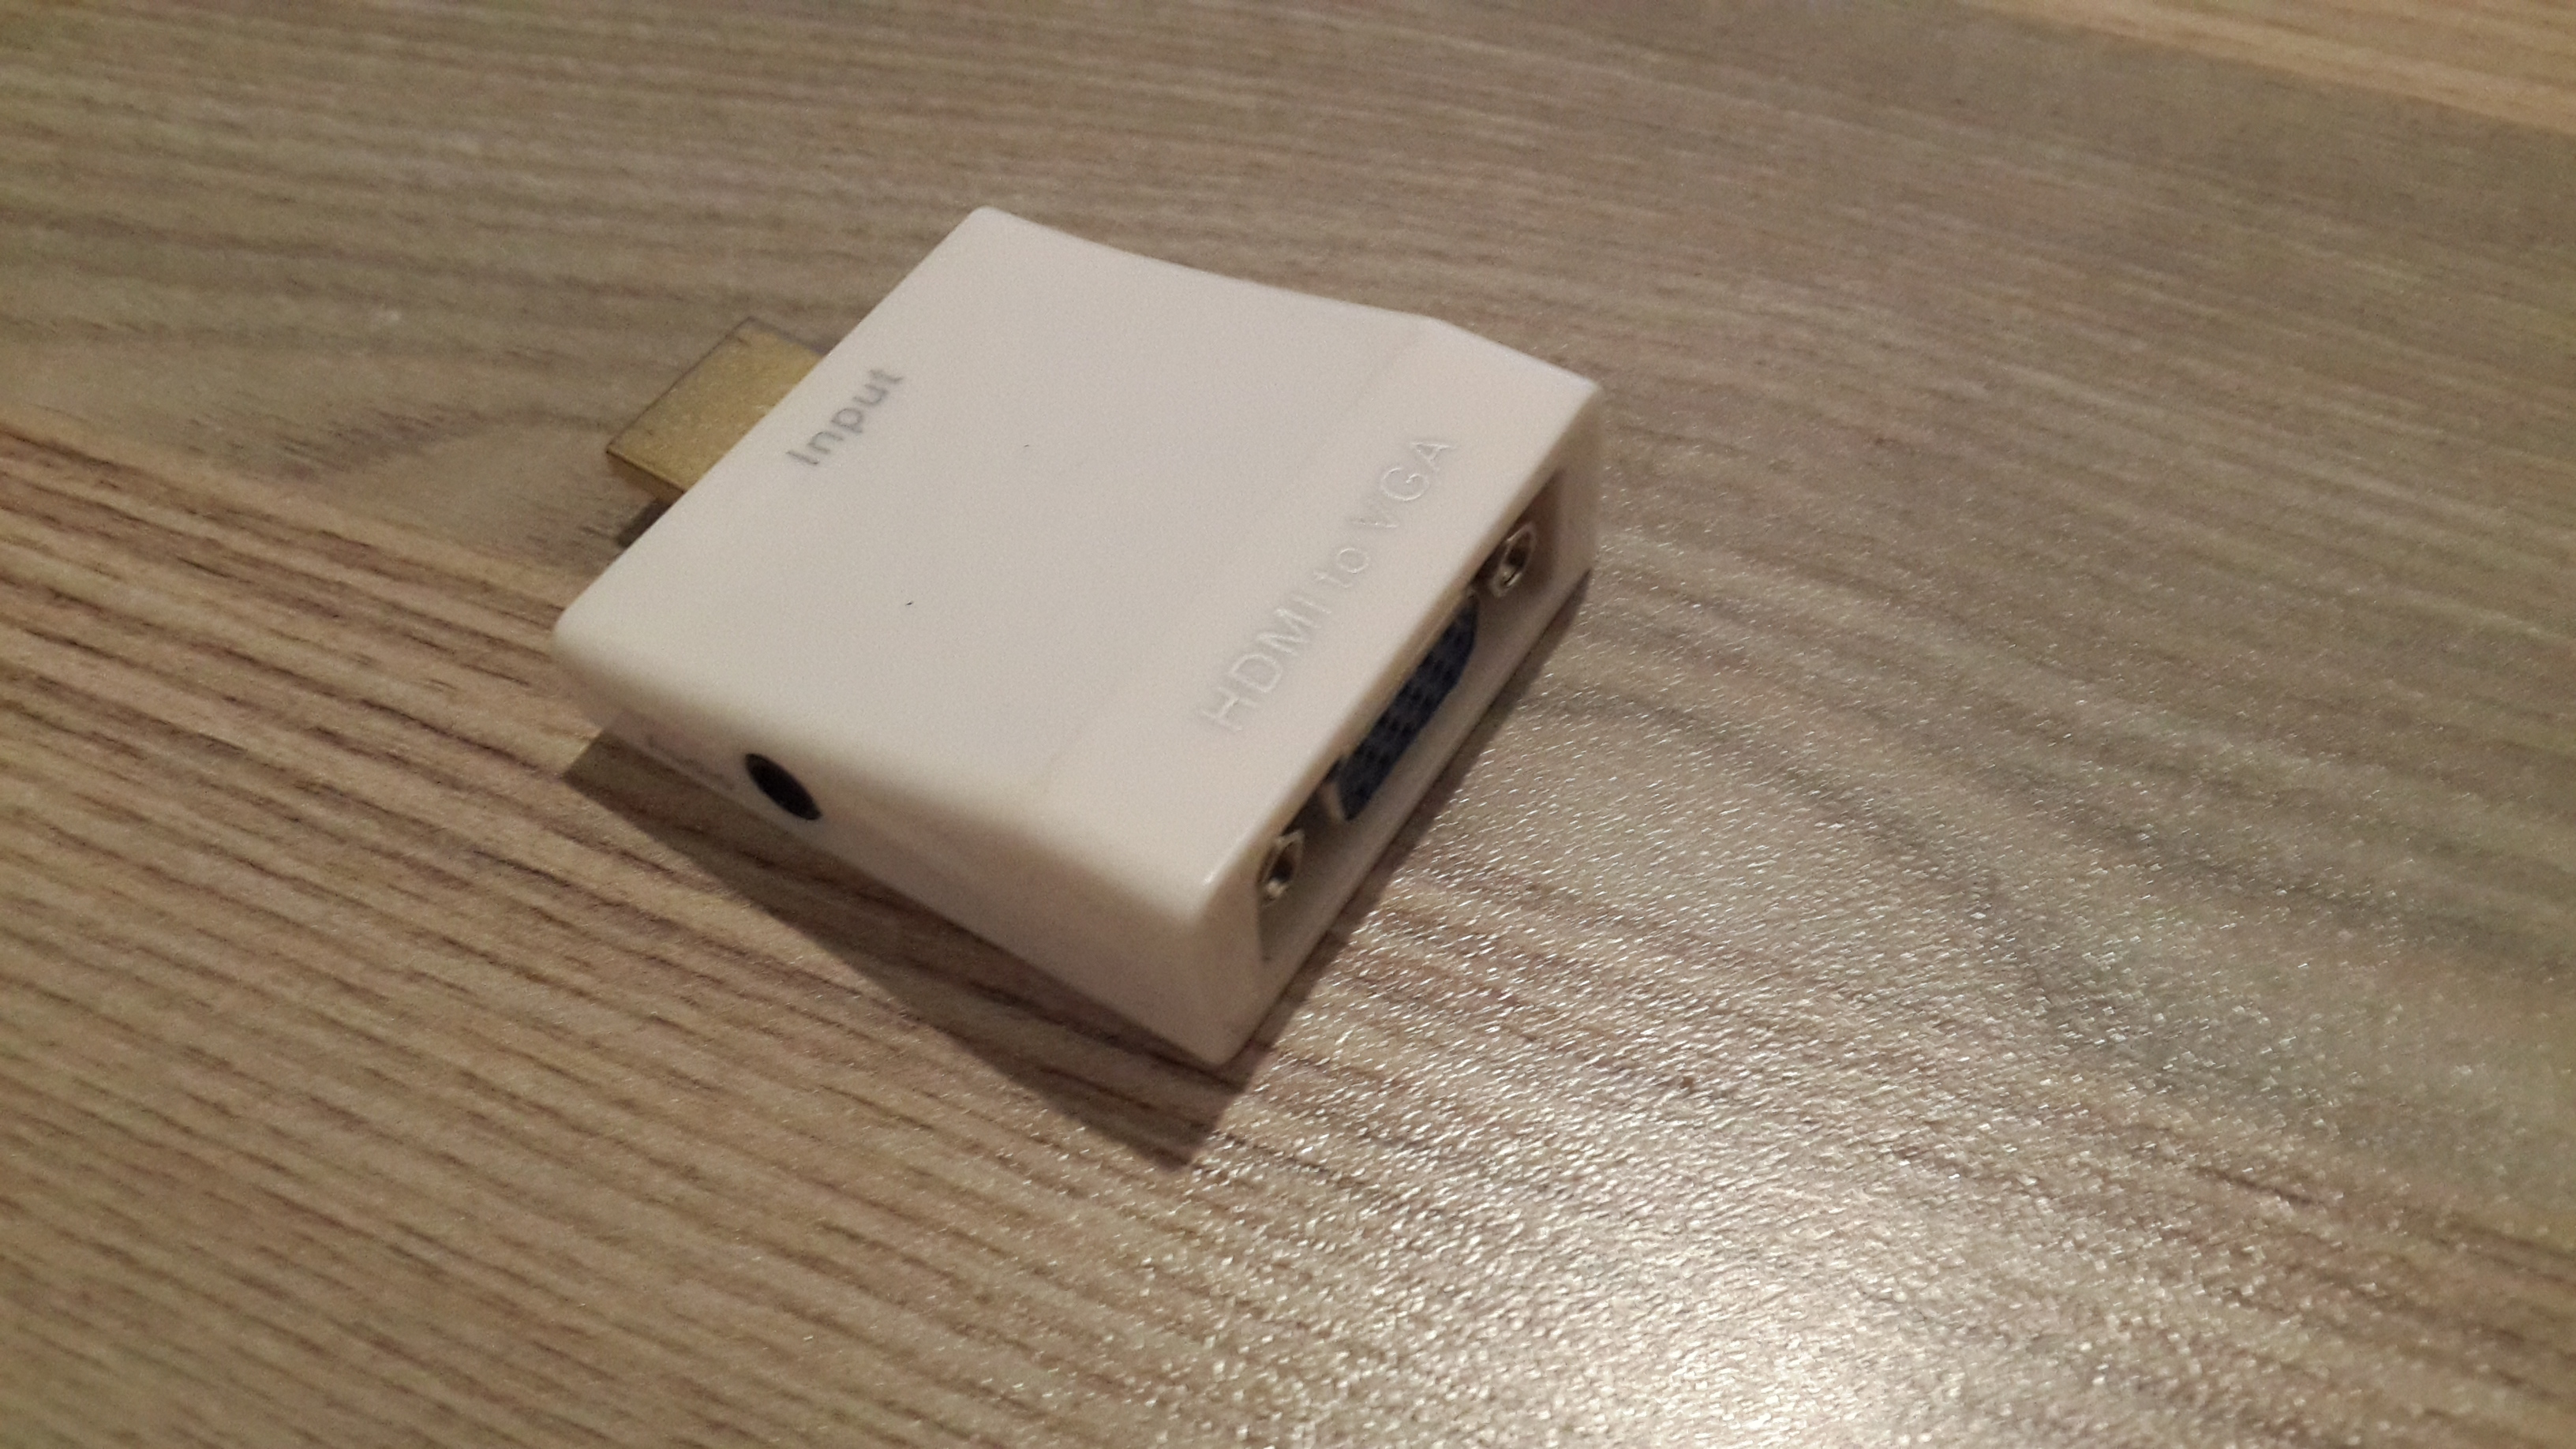
\includegraphics[width=0.9\linewidth]{../images/manual/converter.jpg}
  \caption{ HDMI to VGA Converter}
\end{minipage}
\end{figure}




\begin{figure}[ht!]
\centering
\begin{minipage}{.5\textwidth}
  \centering
 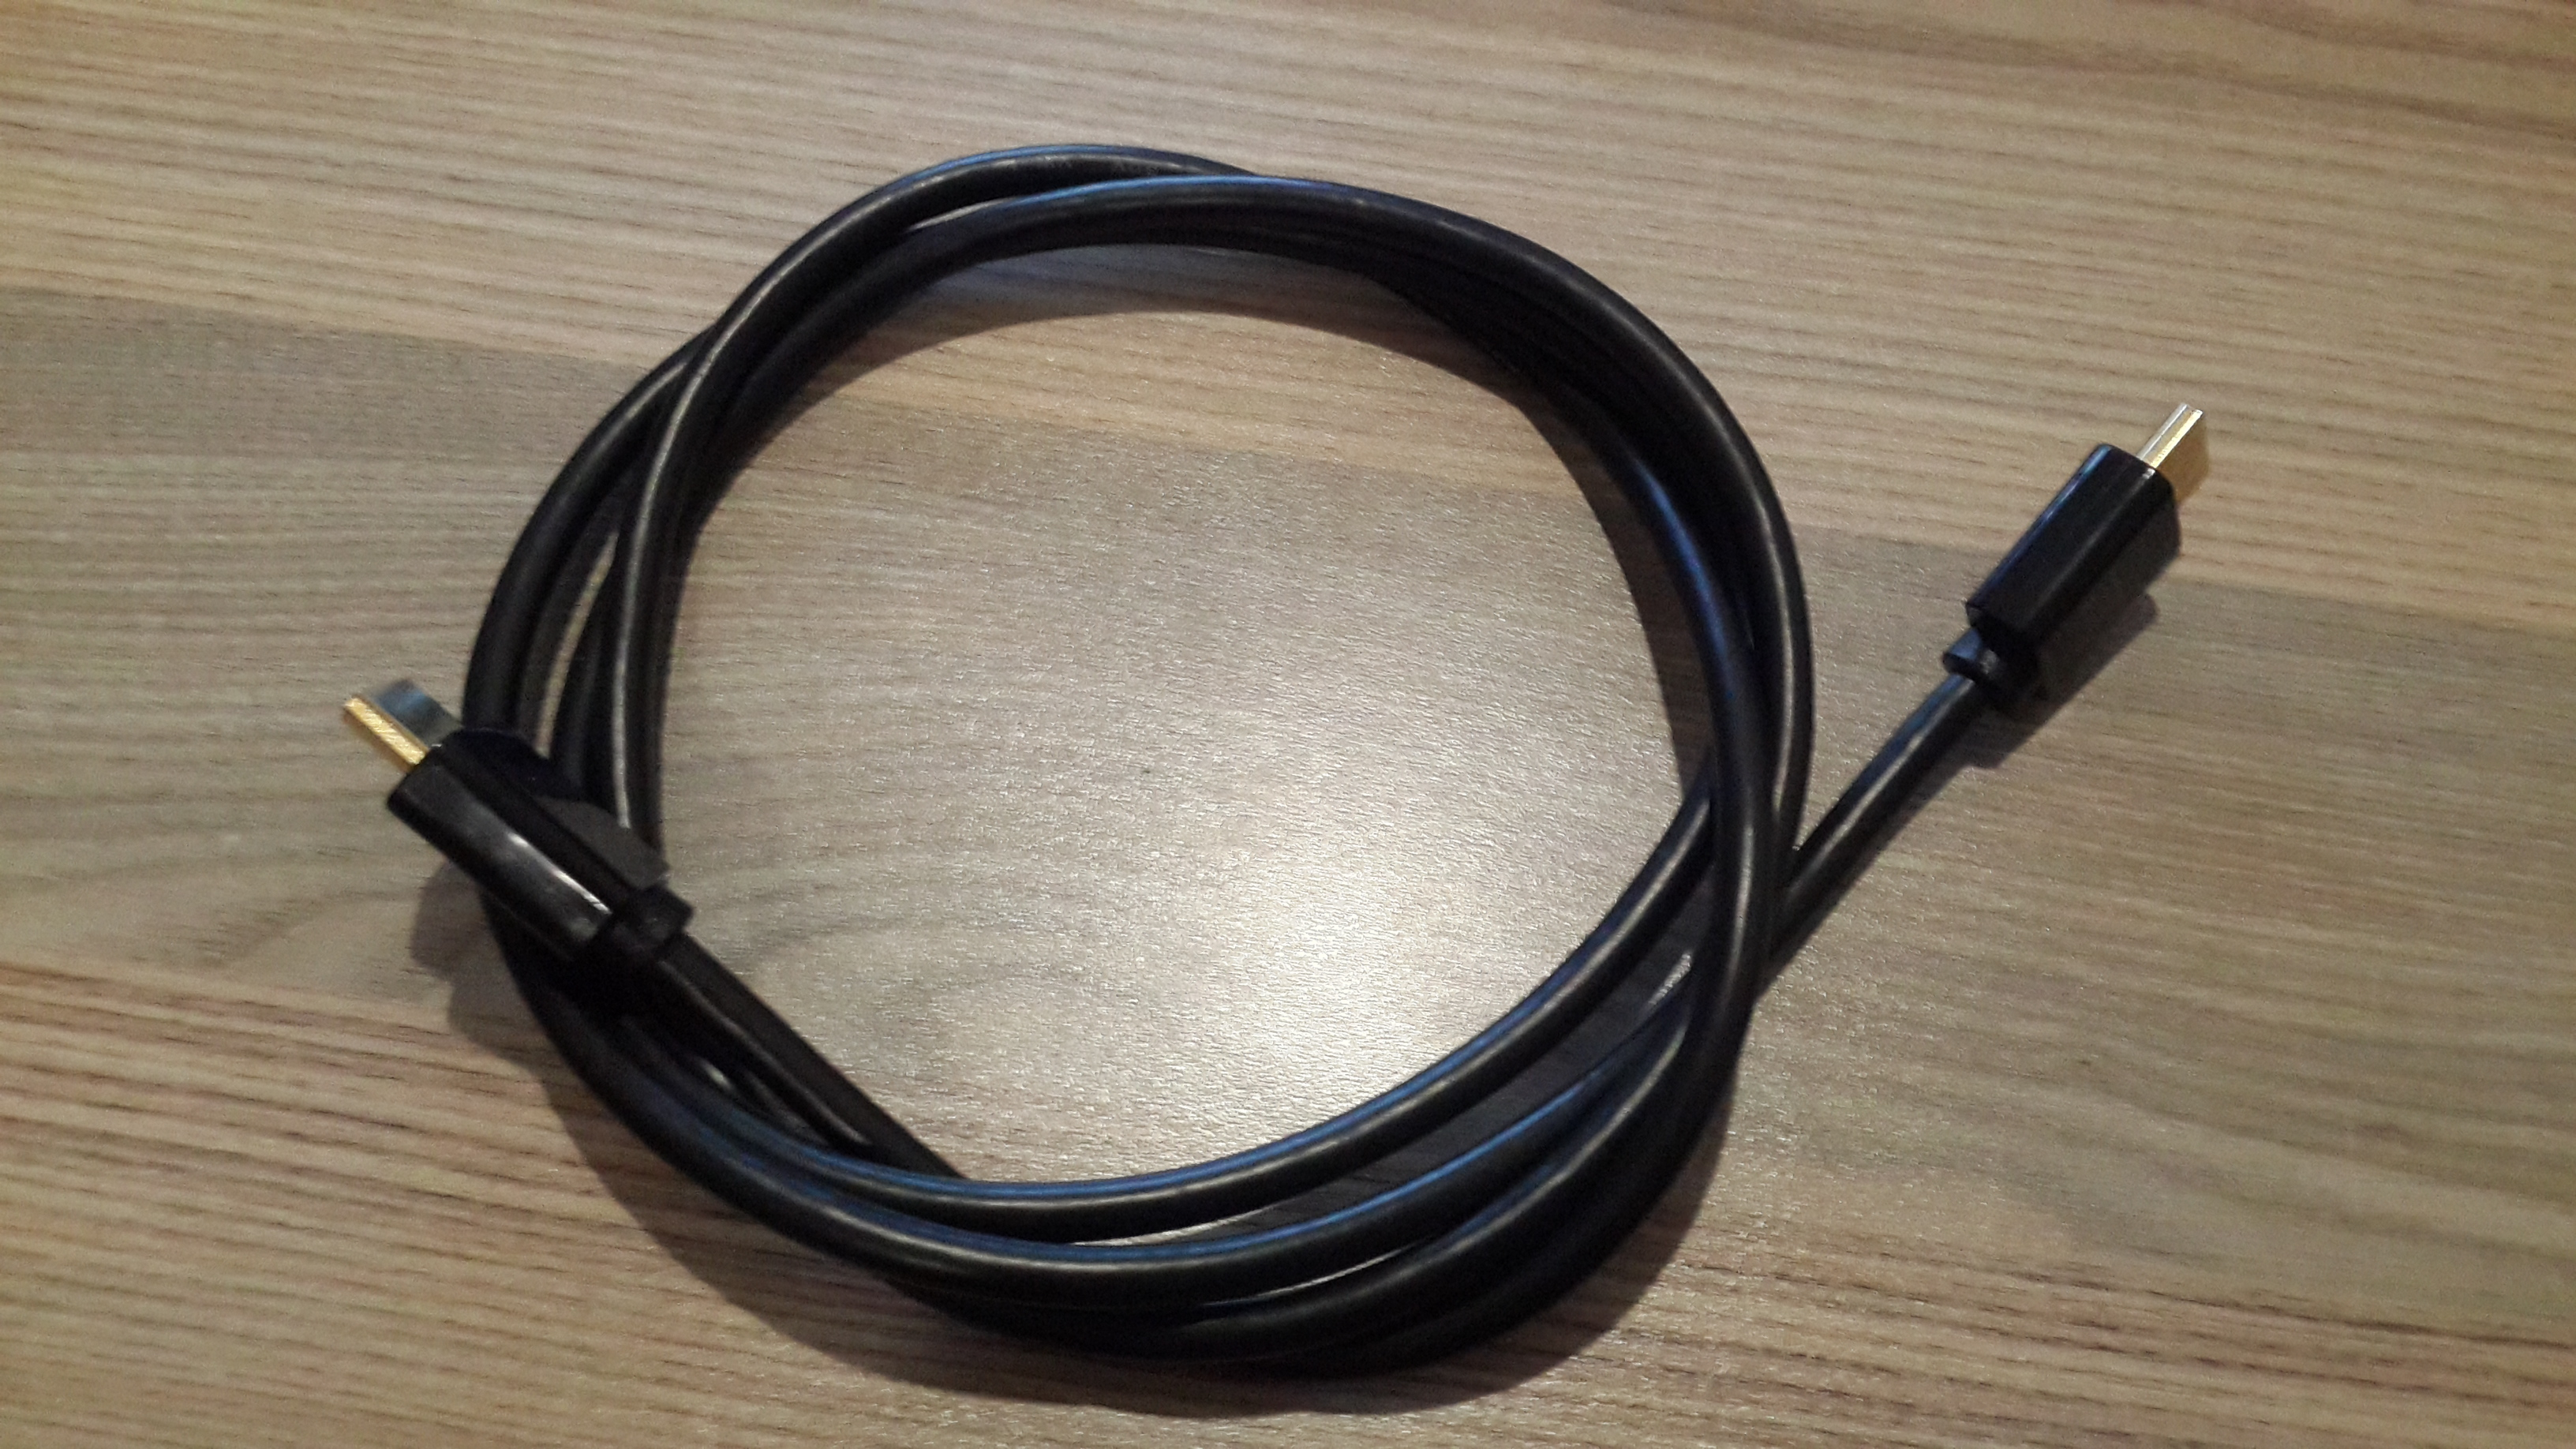
\includegraphics[width=0.9\linewidth]{../images/manual/cable.jpg}
  \caption{ HDMI to HDMI cable}
\end{minipage}
\end{figure}
	\subsection*{\\Steps to set up Raspberry Pi:\\}
		\begin{itemize}
			\item Ensure that there is a WiFi connection in the room that the Pi is to be installed in.
			\item Set up the screen.\\ -Will require a connection to the Raspberry Pi through one of the above mentioned cables.\\-Will be required to be Connected to a power outlet.
			\item Connect the mouse to the Raspberry Pi.
			\item Connect the Raspberry Pi charger to a power outlet and then to the Raspberry Pi.
			\item The Raspberry Pi will power on automatically and start up images should appear on the screen if all steps were followed correctly.
	
			\item Select the internet icon on the top right of the screen.
\begin{figure}[ht!]
\centering
\begin{minipage}{.9\textwidth}
  \centering
 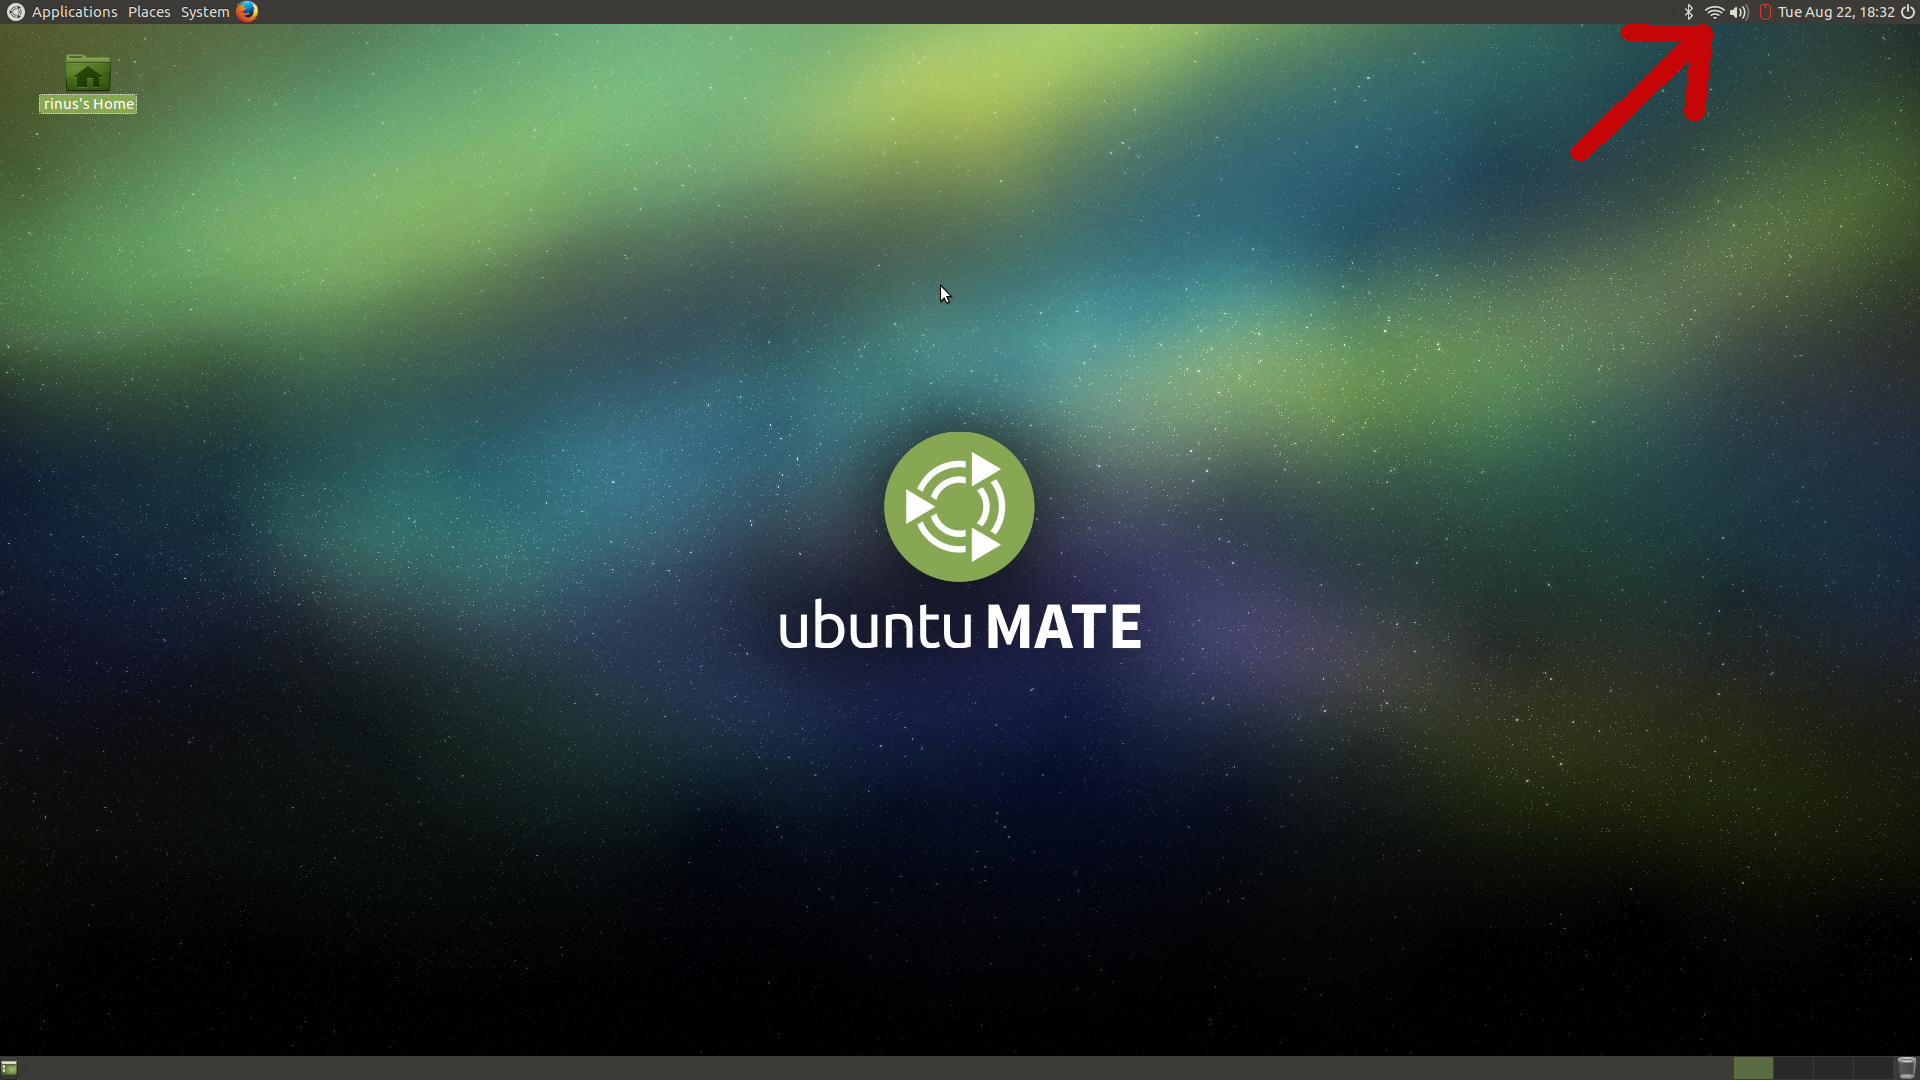
\includegraphics[width=1.0\linewidth]{../images/manual/Desktop.png}
\end{minipage}
\end{figure}
			\item Ensure that both the internet and WiFi are enabled.
			\item Select the Wifi connection that you will be using.
\begin{figure}[ht!]
\centering
\begin{minipage}{.9\textwidth}
  \centering
  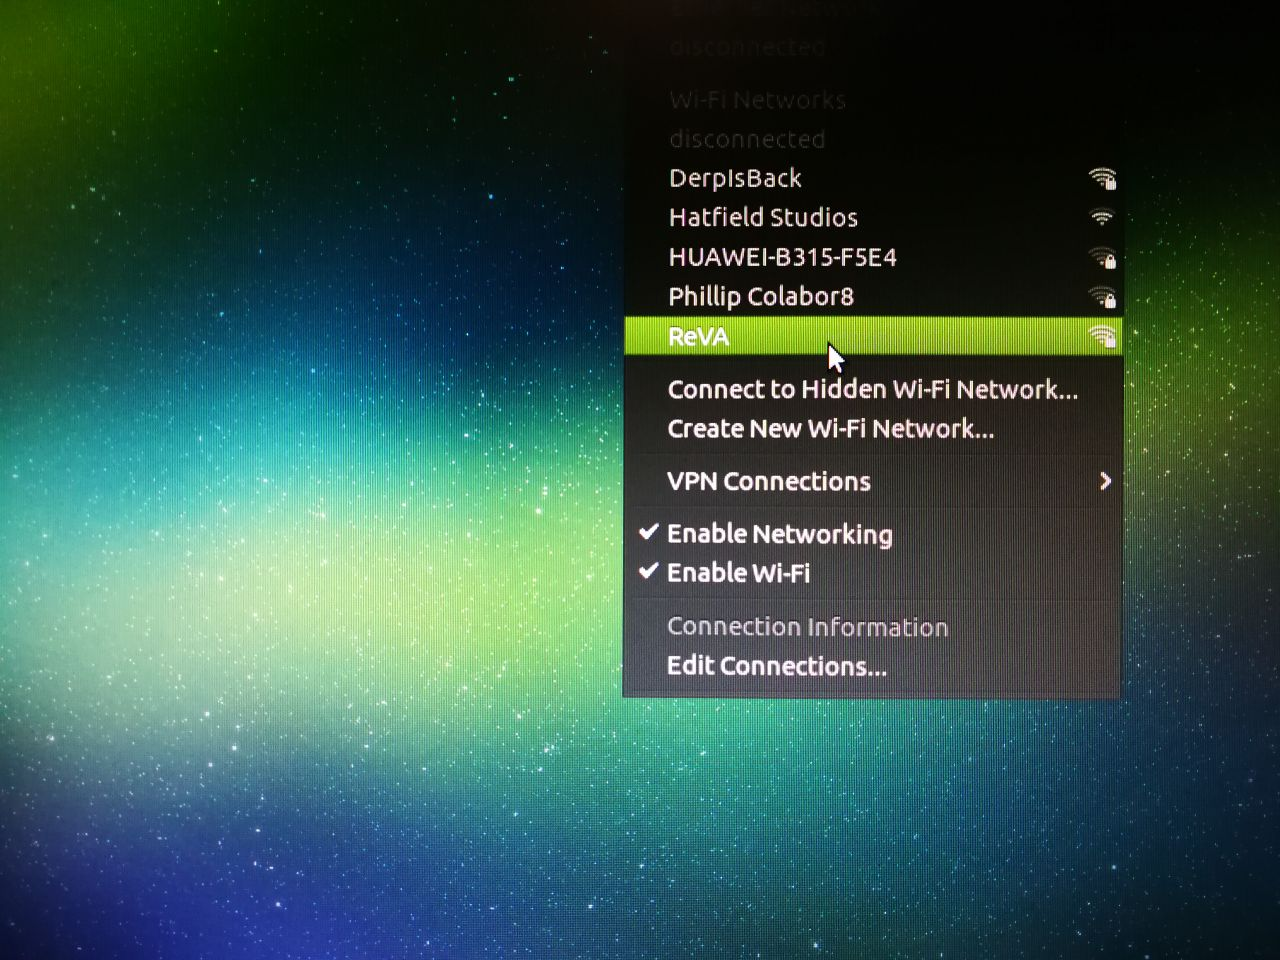
\includegraphics[width=1.0\linewidth]{../images/manual/WifiList.jpg}
\end{minipage}
\end{figure}
			\item Enter in the correct details.
\begin{figure}[ht!]
\centering
\begin{minipage}{.9\textwidth}
  \centering
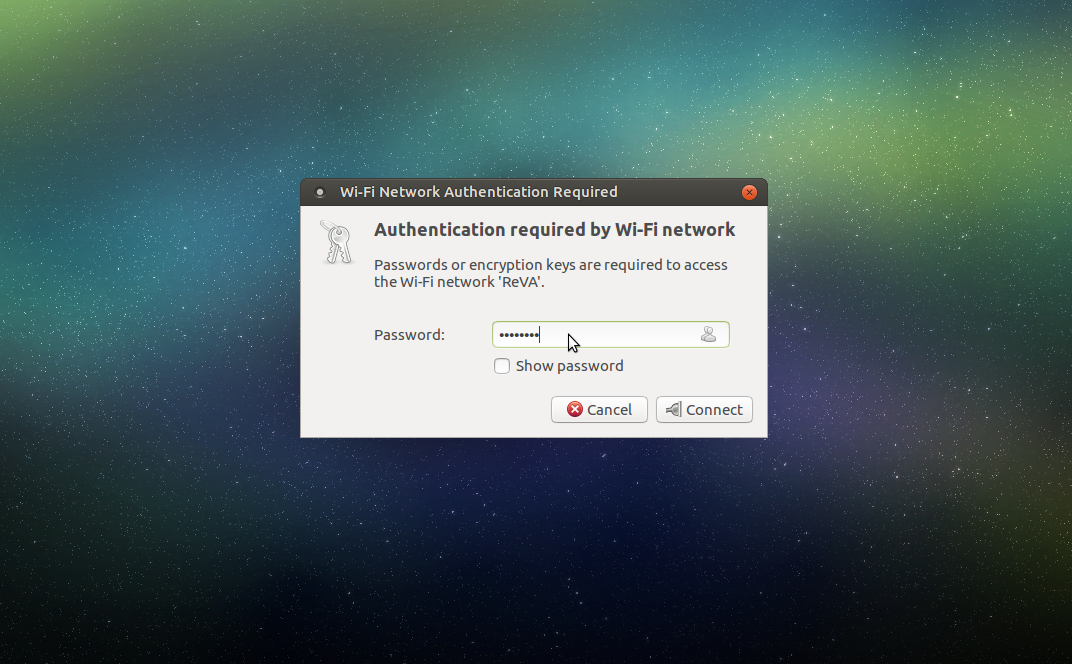
\includegraphics[width=1.0\linewidth]{../images/manual/WifiLogin.png}
\end{minipage}
\end{figure}
			\item You should now be connected to the internet.
\begin{figure}[ht!]
\centering
\begin{minipage}{.9\textwidth}
  \centering
  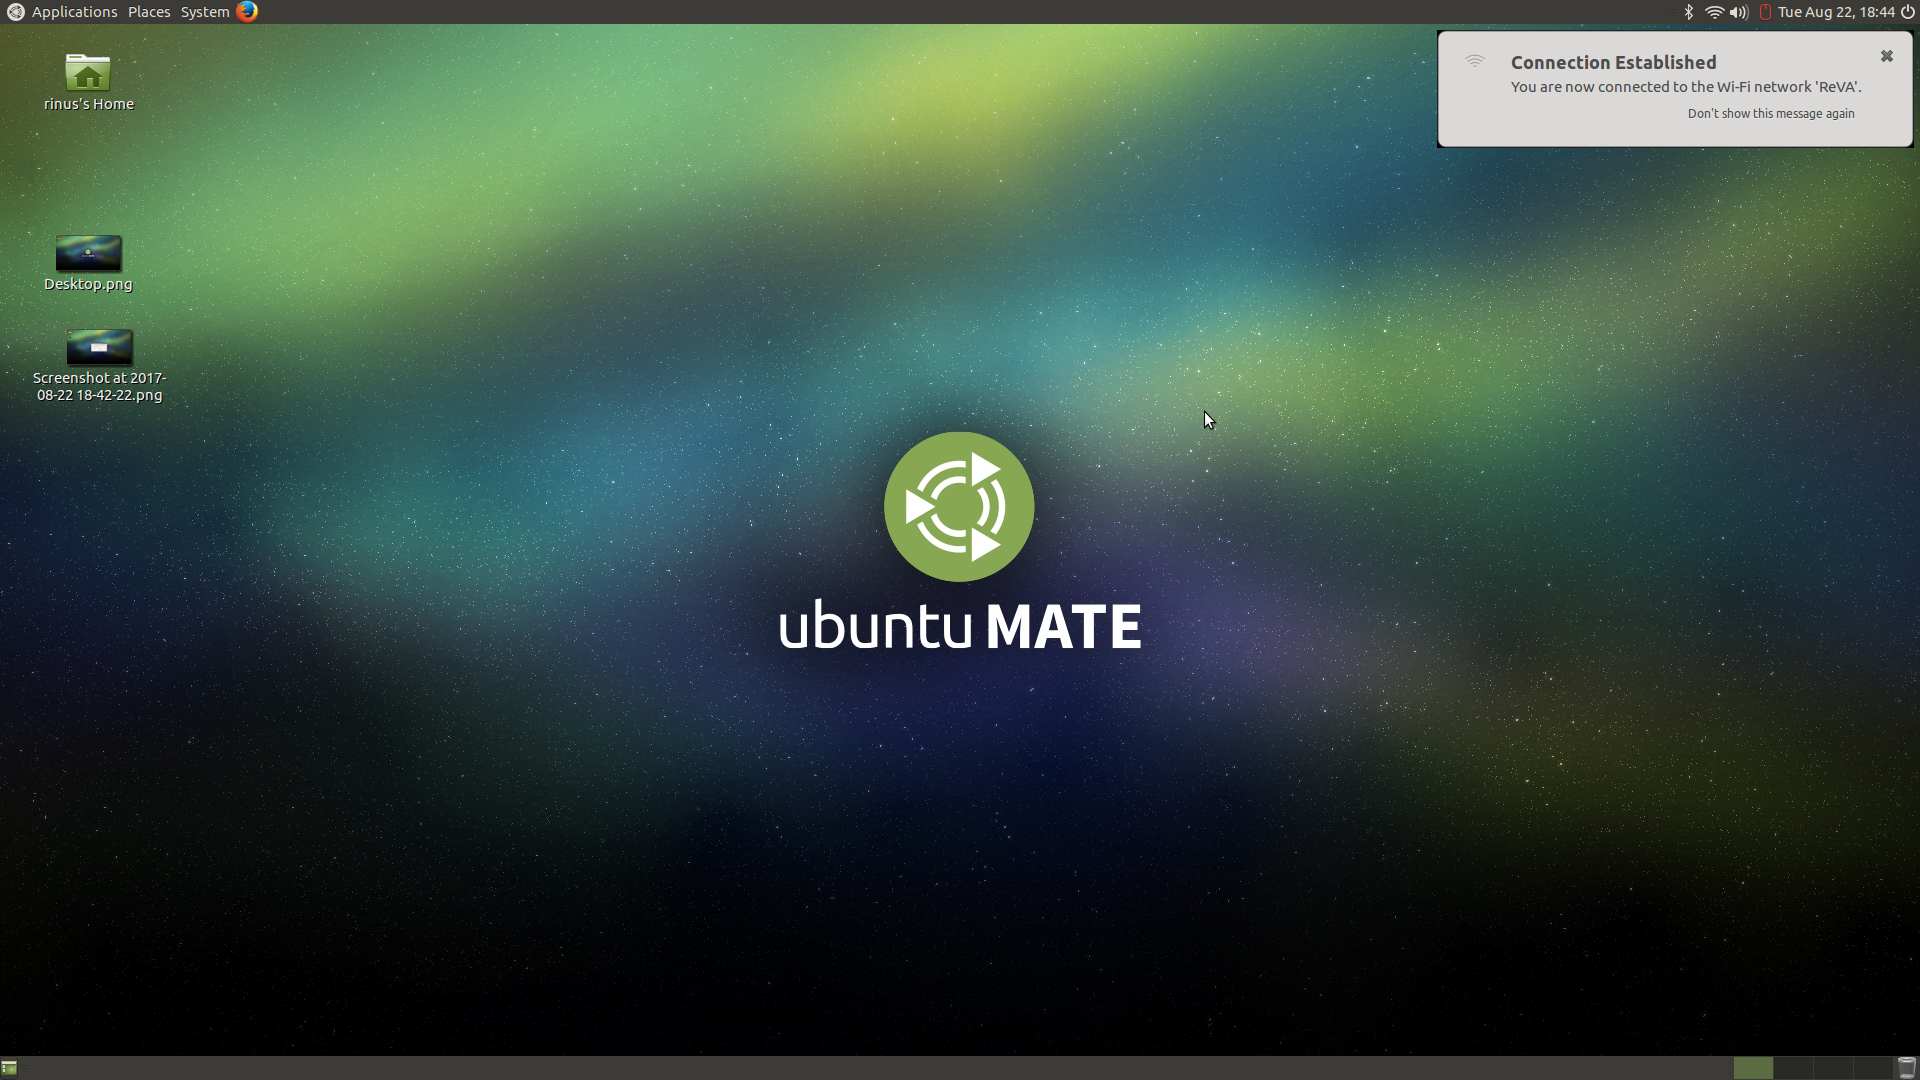
\includegraphics[width=1.0\linewidth]{../images/manual/connection.png}
\end{minipage}
\end{figure}
			\item The screen, mouse and keyboard are no longer needed and can be disconnected. DO NOT Disconnect the Raspberry Pi.
			\textbf{\\\\In the event that the Raspberry Pi is switched off: }
			
			\item Turn off the power to the Raspberry Pi.
			\item Turn the power back on. The device should boot up again and will automatically connect to the internet.
			\textbf{\\\\In the event that the internet connection changes: }
			\item You will have to go through the set up process from the start.
		\end{itemize}


	\subsection*{\\Unsure if Raspberry Pi Server is running?\\}
	
			\begin{itemize}
			\item Connect the screen, keyboard and mouse to the Raspberry Pi.
			\item Power on the Pi as per the above mentioned steps.
			\item Hold CTRL + ALT and press T to open a terminal.
			\item In the terminal type the command top.
			\item Scroll through the running processes looking for a process that says "node" in the right most column.
			\item If the process exists, copy its process ID.\\
				-Press CTRL + C and then enter "kill [Process ID]" and continue following the steps. \\ - If it is not there then continue following the steps.
			\item Open the file explorer.
			\item navigate to \textbackslash Home\textbackslash Reva\textbackslash Zettalet
			\item Right click in the folder.
			\item Select "Open terminal here".
			\item Type "node zettalet" at the terminal prompt.
			\item You have successfully started the server.
		\end{itemize}
		
		

	\subsection*{\\Devices:\\}
		The Libilium MySignals eHealth kit pools the device data. Some of the sensors that can be attached to this computer include: 
		\begin{itemize}
			\item Pulse Oximeter.
			\item Sprirometer.
			\item ECG Sensor.
			\item Blood Pressure Sensor. 
			\item Glucometer.
			\item Scale.
		\end{itemize}
		
\begin{figure}[ht!]
\centering
\begin{minipage}{.9\textwidth}
  \centering 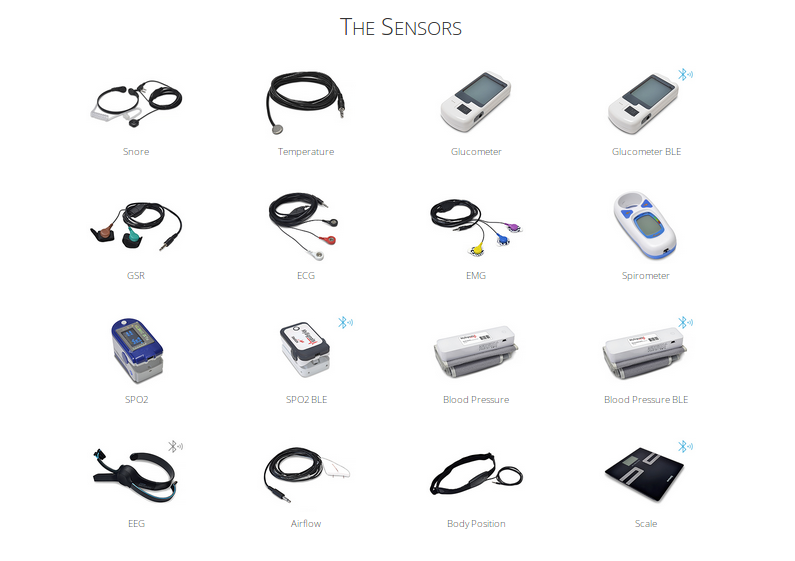
\includegraphics[width=1.0\linewidth]{../images/manual/sensors.png}
 \caption{This image was taken from \href{http://www.my-signals.com/} {here}, the official MySignals website. }
\end{minipage}
\end{figure}
%list of supported devices
%adding a device
%switching on device
%starting server
%developer
%other user?
